\documentclass[11pt,letterpaper]{article}
\PassOptionsToPackage{hyphens}{url}
\usepackage[margin=.83in,top=.8in,bottom=.8in,headheight=15pt]{geometry}
\usepackage[T1]{fontenc}
\usepackage{lmodern,amsmath,amssymb,mathtools,bm,booktabs,array,graphicx,tikz}
\usetikzlibrary{arrows.meta,positioning,calc,decorations.pathreplacing,patterns}
\definecolor{ink}{HTML}{17344D}\definecolor{accent}{HTML}{087E8B}\definecolor{pale}{HTML}{EDF5F5}\definecolor{gold}{HTML}{AD6B19}
\providecommand{\dd}{\,\mathrm{d}}\providecommand{\R}{\mathbb{R}}
\providecommand{\E}{\mathbb{E}}\providecommand{\Var}{\operatorname{Var}}
\providecommand{\Cov}{\operatorname{Cov}}\providecommand{\diag}{\operatorname{diag}}
\providecommand{\norm}[1]{\left\lVert#1\right\rVert}
\providecommand{\abs}[1]{\left|#1\right|}
\usepackage{microtype,hyperref,fancyhdr,enumitem,amsthm,sectsty,needspace}
\allsectionsfont{\raggedright}
\hypersetup{colorlinks=true,linkcolor=ink,urlcolor=accent,pdfauthor={Zan Ahmad},pdftitle={Finite-population genetics: inheritance, drift, and fixation / Lecture notes}}
\setlength{\parindent}{0pt}\setlength{\parskip}{6pt}\linespread{1.07}
\setlist{itemsep=3pt,topsep=4pt,leftmargin=*}
\emergencystretch=2em\clubpenalty=10000\widowpenalty=10000
\pagestyle{fancy}\fancyhf{}\fancyhead[L]{\small Mathematical Modeling}\fancyhead[R]{\small Lecture 7}
\fancyfoot[L]{\footnotesize Zan Ahmad}\fancyfoot[R]{\footnotesize\thepage}\renewcommand{\headrulewidth}{.3pt}
\newtheorem{proposition}{Proposition}\newtheorem{theorem}{Theorem}\newtheorem{lemma}{Lemma}
\theoremstyle{definition}\newtheorem{definition}{Definition}\newtheorem{example}{Example}
\numberwithin{equation}{section}
\begin{document}
{\small\scshape Mathematical Modeling\hfill Lecture 7}\par\medskip
{\raggedright\hyphenpenalty=10000\exhyphenpenalty=10000\LARGE\bfseries\color{ink} Finite-population genetics: inheritance, drift, and fixation\par}\medskip
{\small Lecture notes}\par\bigskip
Genotype probabilities describe random pairing, while a binomial transition describes the sampling of a finite gene pool. We derive both, then use conditional moments to explain how an unchanged mean can coexist with drift, loss of heterozygosity, and eventual fixation.

\section{Allele counts and genotype frequencies}
\hypertarget{note-allele-counts-and-genotype-frequencies}{}\label{note:allele-counts-and-genotype-frequencies}
{\small \href{slides.html\#frame=diploid-accounting\&step=1}{Slides for this section}}\par
Consider a diploid population with $N$ individuals and two alleles, $A$ and $B$, at one locus. The genotype counts satisfy $n_{AA}+n_{AB}+n_{BB}=N$. Each individual contributes two allele copies, so the frequency of $A$ is
\[
p=\frac{2n_{AA}+n_{AB}}{2N},\qquad 1-p=\frac{2n_{BB}+n_{AB}}{2N}.
\]
An allele frequency is not a genotype frequency: heterozygotes contribute one copy of each allele. For example, $(n_{AA},n_{AB},n_{BB})=(10,40,50)$ gives $p=(20+40)/200=0.30$ even though only $10\%$ of individuals are $AA$.

The population size is fixed across discrete, nonoverlapping generations. Our neutral model has no selection, mutation, or migration, and samples offspring copies independently from a common parental pool. These are definitions of the sampling model, not universal descriptions of reproduction. They make it possible to separate random sampling effects from systematic changes in allele frequency.
\section{Random pairing and Hardy--Weinberg probabilities}
\hypertarget{note-random-pairing-and-hardy-weinberg-probabilities}{}\label{note:random-pairing-and-hardy-weinberg-probabilities}
{\small \href{slides.html\#frame=independent-gamete-pairing-figure\&step=1}{Slides for this section}}\par
If the two gametes forming an individual are independent and each carries $A$ with probability $p$, multiplication of probabilities gives
\[
\Pr(AA)=p^2,\qquad \Pr(AB)=2p(1-p),\qquad \Pr(BB)=(1-p)^2.
\]
The factor two counts the two ordered gamete outcomes $(A,B)$ and $(B,A)$ that produce the same heterozygous genotype. Their sum is $(p+1-p)^2=1$. At $p=0.30$ the three probabilities are $0.09$, $0.42$, and $0.49$. Among $100$ independently formed offspring the expected genotype counts are $9$, $42$, and $49$, not compulsory integer outcomes of every sample.

The expected offspring allele frequency is
\[
p^2+\tfrac12\,2p(1-p)=p.
\]
This identity concerns an expectation under the stated pairing assumptions. It does not say that finite-population allele counts are unchanged in each generation. Nor do Hardy--Weinberg probabilities themselves encode dominance, phenotype, or fitness. Those require additional biological definitions.
\begin{center}\begin{minipage}{.98\linewidth}\centering
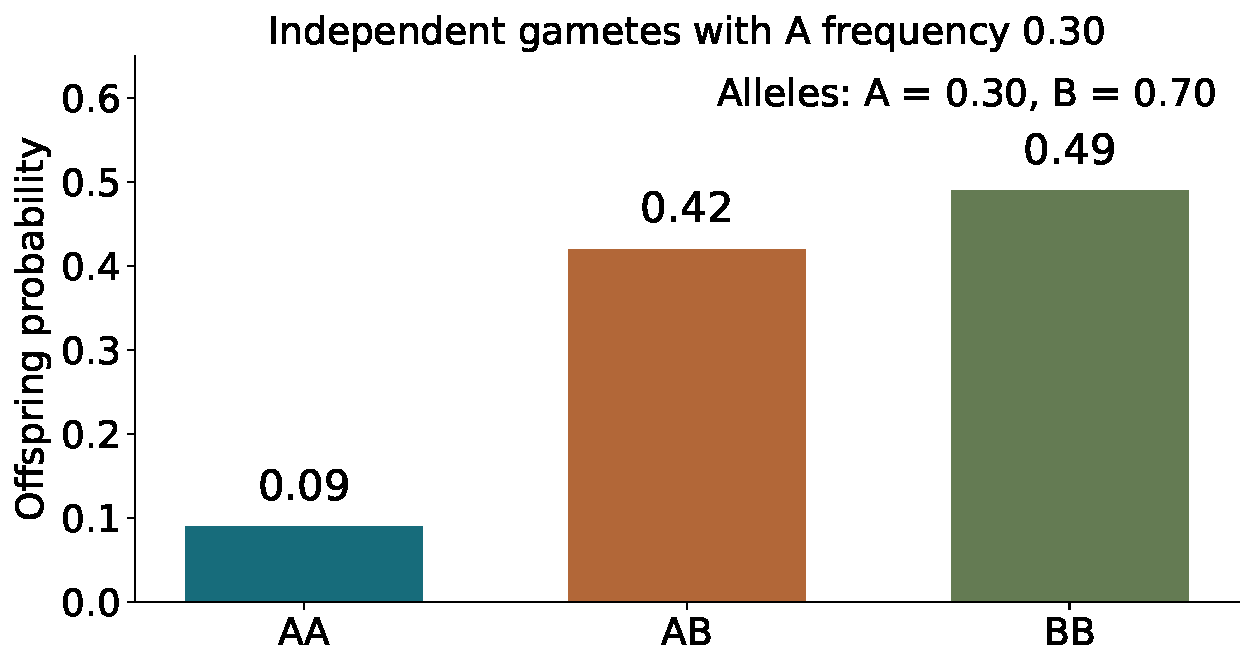
\includegraphics[width=.96\linewidth,height=.57\textheight,keepaspectratio]{genotype-probabilities.pdf}\par\smallskip
{\small Independent gametes with p =\allowbreak{} 0.30 give probabilities 0.09, 0.42 and 0.49 for AA, AB and BB. Finite-population counts can differ from their expectations.}
\end{minipage}\end{center}
\section{The neutral finite-population transition law}
\hypertarget{note-the-neutral-finite-population-transition-law}{}\label{note:the-neutral-finite-population-transition-law}
{\small \href{slides.html\#frame=a-finite-state-variable\&step=1}{Slides for this section}}\par
Let $K_n$ be the number of $A$ copies in generation $n$ and $p_n=K_n/(2N)$. Sampling $2N$ offspring copies independently with replacement from the parental pool gives
\[
K_{n+1}\mid K_n=i\sim\operatorname{Binomial}\!\left(2N,\frac{i}{2N}\right).
\]
Consequently, the transition probabilities of this finite Markov chain are
\[
P_{ij}=\binom{2N}{j}\left(\frac{i}{2N}\right)^j
\left(1-\frac{i}{2N}\right)^{2N-j},\quad 0\leq i,j\leq2N.
\]
At $i=0$ define $P_{00}=1$; at $i=2N$ define $P_{2N,2N}=1$. These absorbing boundary rules avoid ambiguous endpoint expressions such as $0^0$ and state the biological assumption that an absent allele cannot reappear without mutation or migration.

For $N=25$ and $K_n=15$, $p_n=0.30$. A sampled value $K_{n+1}=18$ gives $p_{n+1}=0.36$. This is compatible with neutral sampling. A single increase is not evidence that allele $A$ has a selective advantage. The next draw must use $0.36$, rather than repeatedly drawing from the initial $0.30$ pool.
\section{Conditional moments and accumulation of drift}
\hypertarget{note-conditional-moments-and-accumulation-of-drift}{}\label{note:conditional-moments-and-accumulation-of-drift}
{\small \href{slides.html\#frame=conditional-expectation-and-variance\&step=1}{Slides for this section}}\par
The binomial mean and variance give
\[
\mathbb E[p_{n+1}\mid p_n]=p_n,\qquad
\operatorname{Var}(p_{n+1}\mid p_n)=\frac{p_n(1-p_n)}{2N}.
\]
Thus $p_n$ is a martingale: conditioned on the current population, the mean next frequency is the current one. Iterated expectation gives $\mathbb E[p_n]=p_0$ for a fixed initial frequency. The mean can remain fixed while individual paths fluctuate and their distribution broadens.

At $p=0.30$, the one-generation standard deviation is $\sqrt{0.21/50}\simeq0.06481$ for $N=25$ and $\sqrt{0.21/500}\simeq0.02049$ for $N=250$. Increasing population size tenfold divides the local standard deviation by $\sqrt{10}$, not ten. This conditional variance depends on the current frequency and vanishes at the absorbing endpoints.

Define $a=1-1/(2N)$. Using the conditional second moment,
\[
\begin{aligned}
\mathbb E[p_{n+1}(1-p_{n+1})\mid p_n]
&=p_n-p_n^2-\frac{p_n(1-p_n)}{2N}\\
&=a\,p_n(1-p_n).
\end{aligned}
\]
Therefore expected heterozygosity $H_n=2p_n(1-p_n)$ obeys
\[
\mathbb E[H_n]=2p_0(1-p_0)a^n,
\qquad \operatorname{Var}(p_n)=p_0(1-p_0)(1-a^n).
\]
These are ensemble statements. Eight plotted trajectories are not the ensemble distribution.
\section{Absorption and fixation probability}
\hypertarget{note-absorption-and-fixation-probability}{}\label{note:absorption-and-fixation-probability}
{\small \href{slides.html\#frame=absorbing-endpoints\&step=1}{Slides for this section}}\par
For this finite chain, every interior state has positive probability of reaching an endpoint in the next generation. There are finitely many interior states, so their one-step absorption probabilities have a positive minimum. The probability of avoiding absorption for $n$ further steps is bounded by a geometric sequence and tends to zero. Thus the chain is eventually absorbed at either $0$ or $1$ with probability one.

Since $0\leq p_n\leq1$ and $\mathbb E[p_n]=p_0$, bounded convergence gives
\[
p_0=\mathbb E[p_\infty]
=\Pr(p_\infty=1).
\]
The probability of fixation of $A$ is its initial frequency, even though no allele is favored by selection. Fixation and loss are consequences of finite sampling and absent reintroduction. This argument does not predict the fixation time of a particular run, and it must be reconsidered when selection, mutation, migration, or changing population size is added.
\section{Simulation, reproducibility, and stochastic verification}
\hypertarget{note-simulation-reproducibility-and-stochastic-verification}{}\label{note:simulation-reproducibility-and-stochastic-verification}
{\small \href{slides.html\#frame=computational-checks-for-a-random-model\&step=1}{Slides for this section}}\par
The supplied experiment follows eight neutral paths for $60$ generations, starting from $p_0=0.30$, for $N=25$ and $N=250$. Each population-size panel uses seed $73$. A fixed seed makes a particular computational example repeatable; it does not make that realization representative or create a deterministic ordering between the two panels. The dashed horizontal line is the theoretical mean $p_0$, not the sample average of the eight paths.

Check that every sampled count is an integer between $0$ and $2N$, every frequency lies on the grid $\{0,1/(2N),\ldots,1\}$, and the endpoints remain absorbing. The normalization $2N$ is essential for a diploid model. Independent repeated draws from a fixed input frequency can check the one-generation mean and variance; a statistical test needs a sampling tolerance, not exact equality with the theoretical moment.

In the notebook, change $N$ while holding the initial frequency and number of generations fixed, and distinguish changes in the distribution from features of one path. A deterministic equation $p_{n+1}=p_n$ captures the neutral mean but removes drift and fixation. Matching an ensemble mean therefore does not demonstrate that a model captures the fluctuations of an individual population.
\begin{center}\begin{minipage}{.98\linewidth}\centering
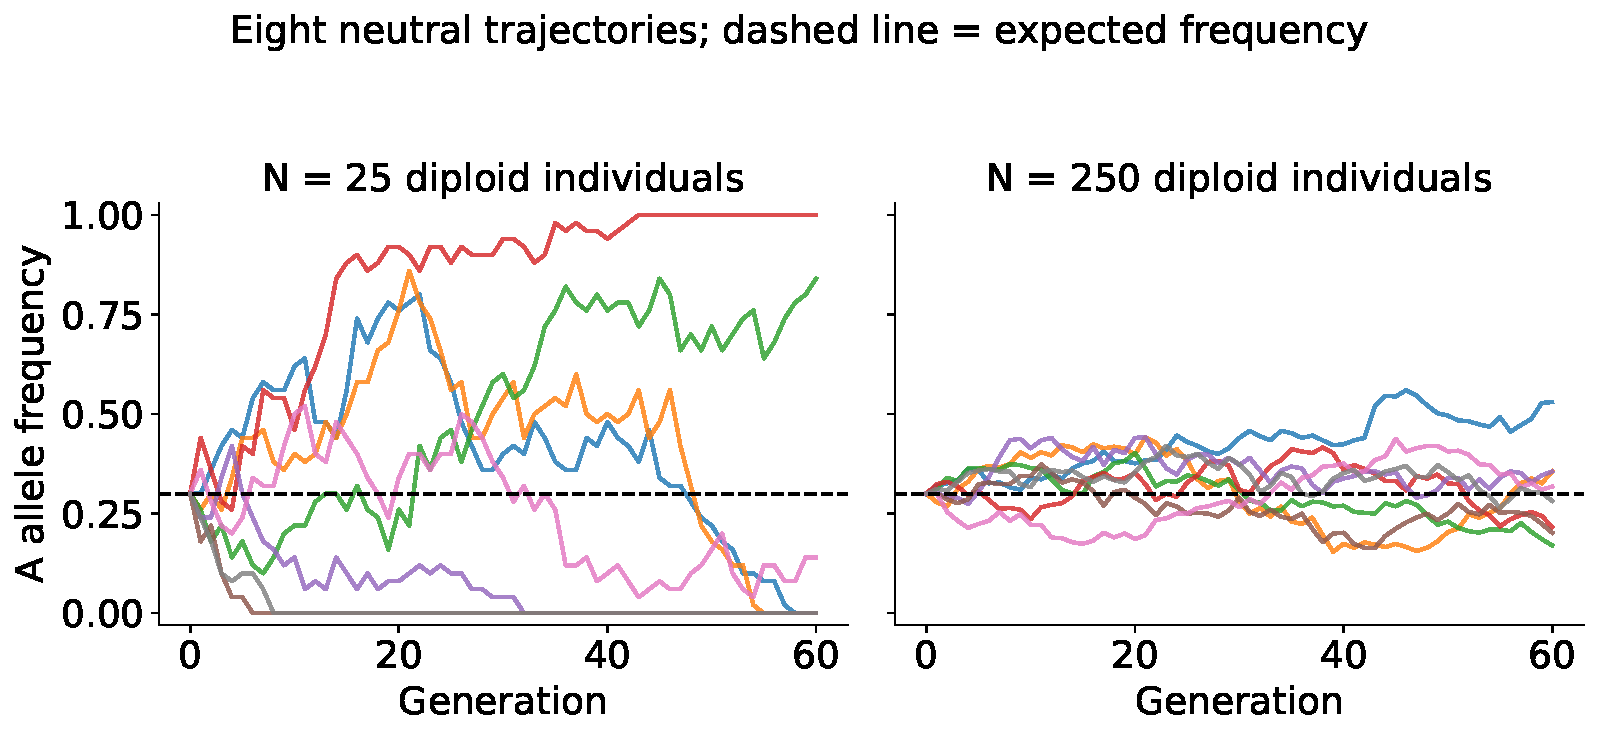
\includegraphics[width=.96\linewidth,height=.57\textheight,keepaspectratio]{neutral-drift.pdf}\par\smallskip
{\small Eight neutral trajectories for N =\allowbreak{} 25 and N =\allowbreak{} 250, each starting at p =\allowbreak{} 0.30. The dashed line is the theoretical expectation, not the average of these eight runs. Both panels use fixed seed 73.}
\end{minipage}\end{center}
\bigskip
\section*{Exercises}
\par\noindent\begin{minipage}{\linewidth}
\subsection*{MM07-E1. Count the right objects}
A diploid census has 12 AA, 26 AB and 12 BB individuals.

\textbf{a} Find N, the total allele-copy count and the A-copy count.

\end{minipage}\par\medskip
\textbf{b} Compute A frequency and observed AB genotype frequency. Are they the same quantity?

\textbf{c} Under independent gamete sampling at this p, predict the next offspring genotype probabilities. Must 50 offspring realize those exact proportions?

\par\noindent\begin{minipage}{\linewidth}
\subsection*{MM07-E2. Account for two mixed orders}
Take p =\allowbreak{} 0.20 and q =\allowbreak{} 0.80.

\textbf{a} Compute AA, AB and BB probabilities and verify their sum.

\end{minipage}\par\medskip
\textbf{b} Give expected genotype counts among 100 independent offspring.

\textbf{c} A proposed calculation uses pq for AB. Show the missing probability and explain the error.

\par\noindent\begin{minipage}{\linewidth}
\subsection*{MM07-E3. Separate one outcome from an expectation}
Use N =\allowbreak{} 25 and initial A copies 15. One next generation contains 18 A copies.

\textbf{a} Compute the initial and next frequencies and the realized change.

\end{minipage}\par\medskip
\textbf{b} Compute the expected next count and one-step frequency variance in the neutral model.

\textbf{c} At N =\allowbreak{} 250 and the same p, how does one-step variance change? Does the upward outcome prove selection?

\par\noindent\begin{minipage}{\linewidth}
\subsection*{MM07-E4. Challenge a simulation}
A program claims to implement the stated closed neutral model.

\textbf{a} Predict all future frequencies if it starts with no A copies.

\end{minipage}\par\medskip
\textbf{b} For N =\allowbreak{} 10, can one realized frequency be 0.13? Explain.

\textbf{c} A student repeats the same random seed ten times and calls the identical curves ten independent confirmations. Repair the claim.

\section*{References}
\noindent\begin{minipage}{\linewidth}
Zan Ahmad, Fall 2024 HEART syllabus. PDF pages 1--2.

\end{minipage}\par\medskip
\noindent\begin{minipage}{\linewidth}
Hoppensteadt and Peskin, Modeling and Simulation in Medicine and the Life Sciences, second edition. Printed pages 269--276; PDF pages 280--287 in the supplied copy.

\end{minipage}\par\medskip
\end{document}
